%
%===============>>  ГРУППА 10-1 МОДУЛЬ 8  <<=============
%
\setmodule{8}

%BEGIN_FOLD % ====>>_____ Занятие 1 _____<<====
\begin{class}[number=1]
	\begin{listofex}
		\item Вычислить с помощью метода приведения:
		\[ \sin135\degree;\;\cos240\degree;\;\tg150\degree;\;\ctg220\degree;\;\sin(-220\degree);\;\tg840\degree;\;\cos(-240\degree);\;\sin315\degree \]
		\item Вычислить:
		\begin{tasks}(1)
			\task \( \dfrac{\sqrt{3}}{\sin60\degree}+\dfrac{3}{\sin30\degree} \)
			\task \( \dfrac{17\sin155\degree}{\sin25\degree} \)
			\task \( \dfrac{-2\sin105\degree}{\cos15\degree} \)
			\task \( \sin^215\degree-1+\cos^215 \)
			\task \( -\sqrt{27}\cos30\degree-\sqrt{2}\sin45\degree\ctg60\degree\tg60\degree\)
		\end{tasks}
		\item Вычислить с помощью метода приведения:
		\[ \cos\dfrac{5\pi}{4};\;\sin\dfrac{7\pi}{3};\;\sin\dfrac{3\pi}{2};\;\sin\left( -\dfrac{5\pi}{3} \right);\;\cos\dfrac{7\pi}{6};\;\sin\dfrac{13\pi}{4};\;\sin\left( -\dfrac{7\pi}{6}  \right);\;\cos\dfrac{21\pi}{4} \]
		\item Вычислить:
		\begin{tasks}(2)
			\task \( \dfrac{5\cos29\degree}{\sin61\degree} \)
			\task \( -4\sqrt{3}\cos(-750\degree) \)
			\task \( \dfrac{4\cos146\degree}{\cos34\degree} \)
			\task \( 7\tg13\degree\cdot\tg77\degree \)
			\task \( \dfrac{12}{\sin^227\degree+\cos^2207\degree} \)
			\task \( \dfrac{5\sin98\degree}{\sin49\degree\cdot\sin41\degree} \)
			\task \( -50\tg9\degree\cdot\tg81\degree+31 \)
		\end{tasks}
		\item Найти:
		\begin{tasks}(1)
			\task \( 5\sin\alpha \), \quad если \( \cos\alpha=\dfrac{2\sqrt{6}}{5} \) и \( \alpha\in\left( \dfrac{3\pi}{2}; 2\pi \right) \);
			\task \( 3\cos\alpha \), \quad если \( \sin\alpha=-\dfrac{2\sqrt{2}}{3} \) и \( \alpha\in\left( \dfrac{3\pi}{2}; 2\pi \right) \);
			\task \( 24\cos\alpha \), \quad если \( \sin\alpha=-0,2 \);
			\task \( \sin\left( \dfrac{7\pi}{2}-\alpha \right) \), \quad если \( \sin\alpha=0,8 \) и \( \alpha\in\left( \dfrac{\pi}{2}; \pi \right) \);
		\end{tasks}
	\end{listofex}
\end{class}
%END_FOLD

%BEGIN_FOLD % ====>>_____ Занятие 2 _____<<====
\begin{class}[number=2]
	\begin{listofex}
		\item Найти:
		\begin{tasks}(2)
			\task \( \cos^2(-46\degree)+\sin^2(-46\degree) \)
			\task \( \sin^223\degree+9+\cos^223\degree \)
			\task \( \dfrac{-13\sin126\degree}{\sin54\degree} \)
			\task \( \dfrac{2\sin^221\degree+2\cos^221\degree}{4} \)
			\task \( \dfrac{ 12\sin 11 \degree \cdot \cos 11 \degree }{ \sin 22 \degree } \)
			\task \( \dfrac{ 24 (\sin^2 17 \degree-\cos^217 \degree) }{ \cos 34 \degree } \)
			\task \( \dfrac{ 5 \cos 29 \degree }{ \sin 61 \degree } \)
			\task \( 36 \sqrt{6} \tg \dfrac{ \pi }{ 4 } \sin \dfrac{ \pi }{ 4 } \)
			\task \( 4 \sqrt{2} \cos \dfrac{ \pi }{ 4 } \cos \dfrac{ 7\pi }{3  } \)
			\task \( \dfrac{ 8 }{ \sin \left( \dfrac{ -27\pi }{ 4 } \right) \cos \left( \dfrac{ 31\pi }{ 4 } \right) } \)
		\end{tasks}
		\item Вычислите:
		\begin{tasks}
			%\task \( \tg\alpha \), \quad если \( \dfrac{7\sin\alpha+13\cos\alpha}{5\sin\alpha-17\cos\alpha}=3 \).
			\task \( 5\sin\alpha \), если \( \cos\alpha=\dfrac{2\sqrt{6}}{5} \) и \( \alpha\in\left( \dfrac{3\pi}{2}; 2\pi \right) \);
			\task \( 3\cos\alpha \), если \( \sin\alpha=-\dfrac{2\sqrt{2}}{3} \) и \( \alpha\in\left( \dfrac{3\pi}{2}; 2\pi \right) \);
			\task \( 24\cos\alpha \), если \( \sin\alpha=-0,2 \);
			\task \( \sin\left( \dfrac{7\pi}{2}-\alpha \right) \), если \( \sin\alpha=0,8 \) и \( \alpha\in\left( \dfrac{\pi}{2}; \pi \right) \);
			%\task \( \dfrac{3\cos\alpha-4\sin\alpha}{2\sin\alpha-5\cos\alpha} \), если \( \tg\alpha=3 \).
		\end{tasks}
		%n5 cos1
		\item Найдите корни уравнения: \( \cos \dfrac{ \pi(x-7) }{ 3 } = 0,5 \).  В ответ запишите наибольший отрицательный корень.
		%n5 cos3
		\item Найдите корни уравнения: \( \cos \dfrac{ \pi(2x+9) }{ 3 } = \dfrac{ \sqrt{2} }{ 2 } \).  В ответ запишите наибольший отрицательный корень.
		%n5 tg1
		\item Найдите корни уравнения: \( \tg \dfrac{ \pi x }{ 4 } = -1 \).  В ответ запишите наибольший отрицательный корень.
		%n5 tg2
		\item Найдите корни уравнения: \( \tg \dfrac{ \pi (x+2) }{ 3 } = -\sqrt{3} \).  В ответ запишите наибольший отрицательный корень.
		%n5 sin1
		\item Найдите корни уравнения: \( \sin \dfrac{ \pi x }{ 3 } = 0,5 \).  В ответ запишите наименьший положительный корень.
	\end{listofex}
\end{class}
%END_FOLD

%BEGIN_FOLD % ====>>_ Домашняя работа 1 _<<====
\begin{homework}[number=1]
	\begin{listofex}
		\item Вычислить: %ПРОВЕРИТЬ НА ДУБЛИКАТЫ 111L1
		\begin{tasks}(2)
			\task \( \dfrac{5\cos29\degree}{\sin61\degree} \)
			\task \( -4\sqrt{3}\cos(-750\degree) \)
			\task \( \dfrac{4\cos146\degree}{\cos34\degree} \)
			\task \( 7\tg13\degree\cdot\tg77\degree \)
			\task \( \dfrac{12}{\sin^227\degree+\cos^2207\degree} \)
			\task \( \dfrac{5\sin98\degree}{\sin49\degree\cdot\sin41\degree} \)
			\task \( -50\tg9\degree\cdot\tg81\degree+31 \)
		\end{tasks}
		%n5 cos2
		\item Найдите корни уравнения: \( \cos \dfrac{ \pi(x-1) }{ 3 }=\dfrac{  1}{ 2 } \).  В ответ запишите наибольший отрицательный корень.
		%n5 sin2
		\item Найдите корни уравнения: \( \sin \dfrac{ \pi(4x-3) }{ 4 }=1 \).  В ответ запишите наибольший отрицательный корень.
		%n5 tg3
		%\item Найдите корни уравнения: \( \tg \dfrac{ \pi(x-3) }{ 6 }=\dfrac{ 1 }{ \sqrt{3} } \).  В ответ запишите наибольший отрицательный корень.
		\item Найдите: %6 1-6 9
		\begin{tasks}
			\task \( \tg \alpha \), если \( \cos \alpha = \dfrac{ \sqrt{10} }{ 10 } \) и \( \alpha\in\left( \dfrac{ 3\pi }{ 2 };2\pi \right) \);
			\task \( 26 \cos \left( \dfrac{ 3\pi }{ 2 }+\alpha \right) \), если \( \cos \alpha = \dfrac{ 12 }{ 13 } \) и \( \alpha\in\left( \dfrac{ 3\pi }{ 2 };2\pi \right) \);
			%\task \( \dfrac{ 10\sin 6 \alpha }{ 3 \cos 3 \alpha } \), если \( \sin 3 \alpha = 0,6 \).
		\end{tasks}
	\end{listofex}
\end{homework}
%END_FOLD

%BEGIN_FOLD % ====>>_____ Занятие 3 _____<<====
\begin{class}[number=3]
	\begin{listofex}
			\item Вычислите: %111
		\begin{tasks}(2)
			\task \( \dfrac{ 5\sin 74 \degree }{ \cos 37 \degree \cdot \cos 53 \degree } \)
			\task \( \dfrac{ 23 }{ \sin^2 56 \degree + 1 + \sin^2 146 \degree } \)
			\task \( -\dfrac{ 4 }{ \sin^2 27 \degree + \sin^2 117 \degree } \)
			\task \( -\dfrac{ 4\cos 22,5 \degree \sin 22,5 \degree }{ 8 } \)
			\task \( \dfrac{ 50 \sin 19 \degree \cos 19 \degree }{ \sin 38 \degree } \)
			\task \( \dfrac{ \sin \dfrac{ 3\pi }{8 } \cos \dfrac{ 3\pi }{ 8 } }{ 20 } \)
			\task \( -\dfrac{ 7 }{ \sin^2 \left( \dfrac{ \pi }{ 15 } \right) + \cos^2 \left( \dfrac{ \pi }{ 15 } \right) } \)
			\task \( \cos^2\left( -\dfrac{ 3\pi }{ 8 } \right) +\sin^2\left( -\dfrac{ 3\pi }{ 8 } \right) \)
			\task \( \sin^2 (-88\degree) + \cos^2 (-88\degree) -5 \)
			\task \( \dfrac{2\sin^2 21\degree+2\cos^221\degree}{4} \)
		\end{tasks}
		%\item Найдите: %111
		%\begin{tasks}
		%	\task \( \dfrac{ 10\sin 6 \alpha }{ 3 \cos 3 \alpha } \), если \( \sin 3 \alpha = 0,6 \).
		%\end{tasks}
		%n5 cos1
		\item Найдите корни уравнения: \( \cos \dfrac{ \pi(x-7) }{ 3 } = 0,5 \).  В ответ запишите наибольший отрицательный корень.
		%n5 cos3
		\item Найдите корни уравнения: \( \cos \dfrac{ \pi(2x+9) }{ 3 } = \dfrac{ \sqrt{2} }{ 2 } \).  В ответ запишите наибольший отрицательный корень.
		%n5 tg1
		\item Найдите корни уравнения: \( \tg \dfrac{ \pi x }{ 4 } = -1 \).  В ответ запишите наибольший отрицательный корень.
		%n5 tg2
		\item Найдите корни уравнения: \( \tg \dfrac{ \pi (x+2) }{ 3 } = -\sqrt{3} \).  В ответ запишите наибольший отрицательный корень.
		%n5 sin1
		\item Найдите корни уравнения: \( \sin \dfrac{ \pi x }{ 3 } = 0,5 \).  В ответ запишите наименьший положительный корень.
	\end{listofex}
\end{class}
%END_FOLD

%BEGIN_FOLD % ====>>_____ Занятие 4 _____<<====
\begin{class}[number=4]
	\begin{listofex}
		%n5 cos2
		\item Найдите корень уравнения: \( \cos \dfrac{ \pi(x-1) }{ 3 }=\dfrac{ 1 }{ 2 } \). В ответе запишите наибольший отрицательный корень.
		%n5 cos4
		\item Найдите корень уравнения: \( \cos \dfrac{ \pi(x+1) }{ 4 }=\dfrac{ \sqrt{2} }{ 2 } \). В ответе запишите наименьший положительный корень
		%n5 tg3
		\item Решите уравнение \(\tg \dfrac{ \pi(x-3) }{ 6 }= \dfrac{ 1 }{ \sqrt{3} }\). В ответе напишите наибольший отрицательный корень.
		%n5 tg4
		\item Решите уравнение \(\tg \dfrac{ \pi(4x-5) }{4 }= -1\). В ответе напишите наименьший положительный корень.
		%n5 sin2
		\item Решите уравнение \( \sin \dfrac{ \pi(4x-3) }{ 4 }=1 \). В ответе напишите наибольший отрицательный корень.
		%n5 sin3
		\item Решите уравнение \( \sin \dfrac{ \pi(8x+3) }{ 6 }=0,5 \). В ответе напишите наименьший положительный корень.
		%priklad trigon 1
		\item При нормальном падении света с длиной волны \( \lambda=400 \) нм на дифракционную решeтку с периодом \(d\) нм наблюдают серию дифракционных максимумов. При этом угол \(\varphi\)  (отсчитываемый от перпендикуляра к решeтке), под которым наблюдается максимум, и номер максимума \(k\) связаны соотношением \(d \sin \varphi= k\lambda\). Под каким минимальным углом \(\varphi\) (в градусах) можно наблюдать второй максимум на решeтке с периодом, не превосходящим \(1600\) нм?
		%priklad trigon 2
		\item Два тела массой \(m=2\) кг каждое, движутся с одинаковой скоростью  \(v =10\) м/с под углом \(2\alpha\) друг к другу. Энергия (в джоулях), выделяющаяся при их абсолютно неупругом соударении определяется выражением \(Q= m v^2 \sin^2 \alpha \). Под каким наименьшим углом \(2\alpha\) (в градусах) должны двигаться тела, чтобы в результате соударения выделилось не менее \(50\) джоулей?
		\item Найдите площадь треугольника, две стороны которого равны \(8\) и \(12\), а угол между ними равен \(30 \degree\).
		\item Большее основание равнобедренной трапеции равно \(34\). Боковая сторона равна \(14\). Синус острого угла равен \( \dfrac{ 2\sqrt{10}}{ 7 } \). Найдите меньшее основание.
		\item Основания равнобедренной трапеции равны \(7\) и \(51\). Тангенс острого угла равен \( \dfrac{ 5 }{ 11 } \).  Найдите высоту трапеции.
	\end{listofex}
\end{class}
%END_FOLD

%BEGIN_FOLD % ====>>_ Домашняя работа 2 _<<====
\begin{homework}[number=2]
	\begin{listofex}
		%n5 cos5
		\item Найдите корень уравнения: \( \cos \dfrac{ \pi(8x+1) }{ 6 } = \dfrac{ \sqrt{3} }{ 2 } \). В ответе запишите наибольший отрицательный корень.
		%n5 tg5
		\item Решите уравнение \( \tg \dfrac{ \pi(x+3) }{ 3 }=-\sqrt{3} \). В ответе напишите наибольший отрицательный корень.
		%n5 sin4
		\item Решите уравнение \( \sin \dfrac{ \pi(x+9) }{ 4 }=-\dfrac{ \sqrt{2} }{ 2 } \). В ответе напишите наименьший положительный корень.
		%priklad trigon 3
		\item Катер должен пересечь реку шириной \(L = 100\) м и со скоростью течения \(u =0,5\) м/с так, чтобы причалить точно напротив места отправления. Он может двигаться с разными скоростями, при этом время в пути, измеряемое в секундах, определяется выражением \(t=\dfrac{ L }{ u } \ctg \alpha \) где \(\alpha\) --- острый угол, задающий направление его движения (отсчитывается от берега). Под каким минимальным углом \(\alpha\) (в градусах) нужно плыть, чтобы время в пути было не больше \(200\) с?
		%трапеция N5
		\item Меньшее основание равнобедренной трапеции равно \(23\). Высота трапеции равна \(39\). Тангенс острого угла равен \(\dfrac{ 13 }{ 8 }\). Найдите большее основание.
		%треуг1 N5
		\item В треугольнике \(ABC\): \(AC=BC=7, \tg A = \dfrac{ 33 }{ 4\sqrt{33} }\). Найдите \(AB\).
		%параллелог1 N1
		\item В параллелограмме \(ABCD \): \( AB  =  3, AD  =  21\), \( \sin A = \dfrac{ 6 }{ 7 } \). Найдите большую высоту параллелограмма.
	\end{listofex}
\end{homework}
%END_FOLD

%BEGIN_FOLD % ====>>_____ Занятие 5 _____<<====
\begin{class}[number=5]
	\begin{listofex}
		\item В пачке \(250\) листов бумаги формата \(A4\). За неделю в офисе расходуется \(700\) листов. Какого наименьшего количества пачек бумаги хватит на \(8\) недель.
		\item Установите соответствие между величинами и их возможными значениями: к каждому элементу первого столбца подберите соответствующий элемент из второго столбца. \\ \\
		\begin{minipage}[t]{0.58\linewidth}
			\textbf{Величины:}
			\begin{tasks}
				\task площадь трехкомнатной квартиры
				\task площадь футбольного поля
				\task площадь территории России
				\task площадь купюры достоинством в \(100\) рублей \\
			\end{tasks}
		\end{minipage}
		\hspace{0.05\linewidth}
		\begin{minipage}[t]{\textwidth}
			\textbf{Возможные значения:}
			\begin{tasks}
				\task \( 0,7 \) га
				\task \( 100 \) кв. м
				\task \( 97,5 \) кв. см
				\task \( 17,1 \) млн кв. км
			\end{tasks}
		\end{minipage}
		\item На диаграмме показано количество посетителей сайта РИА «Новости» во все дни с \(10\) по \(29\) ноября \(2009\) года. По горизонтали указываются дни месяца, по вертикали --- количество посетителей сайта за данный день. Определите по диаграмме, какого числа количество посетителей сайта РИА «Новости» было наименьшим за указанный период.
		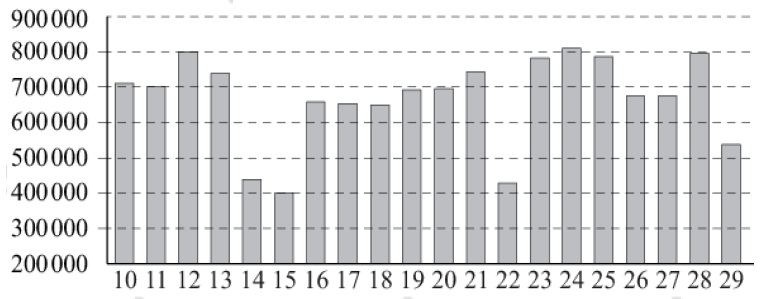
\includegraphics[align=t, width=\linewidth]{../pics/G101M8L5-1}
		\item Площадь четырехугольника можно вычислить по формуле \[S=\dfrac{ 1 }{ 2 }d_1 d_2 \sin \alpha,\] где \(d_1\) и \(d_2\) --- длины диагоналей четырехугольника, \(\alpha\) --- угол между диагоналями. Пользуясь этой формулой, найдите площадь \(S\), если \(d_1=4, d_2 = 7, \sin \alpha = \dfrac{  2}{ 7 }\).
		\item Научная конференция проводится в \(3\) дня. Всего запланировано \(50\) докладов: в первый день --- \(18\) докладов, остальные распределены поровну между днями. Порядок докладов определяется случайным образом. Какова вероятность того, что доклад профессора М. окажется запланированным на последний день конференции?
		\item Независимая экспертная лаборатория определяет рейтинг мясорубок на основе коэффициента ценности, равного \(0,01\) средней цены \(P\) (в рублях), показателей функиональности \(F\), качества \(Q\) и дизайна \(D\). Рейтинг \(R\) вычисляется по формуле: \[ R=3(F+1)+D-0,01P. \] В таблице даны цены и показатели четырех моделей мясорубок:
		\\
		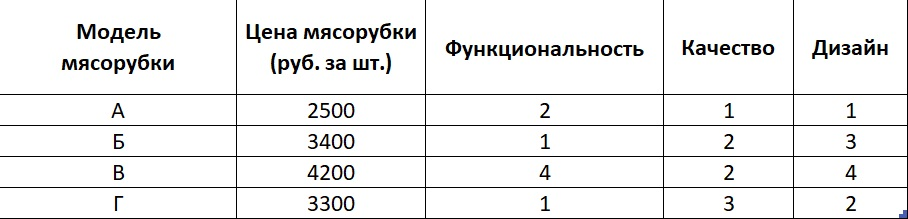
\includegraphics[align=t, width=\linewidth]{../pics/G101M8L5-2}
		\\
		\\ Найдите наивысший рейтинг мясорубки из представленных в таблице.
		\item На рисунках изображены графики функций вида \(y=kx+b\). Установите соответствие между графиками функций и угловыми коэффициентами прямых.
		\\ \textbf{Графики:}
		\\
		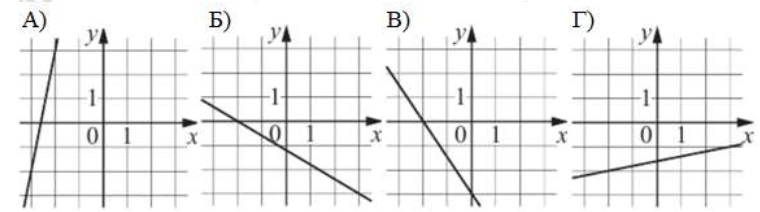
\includegraphics[align=t, width=\linewidth]{../pics/G101M8L5-3}
		\\ \\
		\textbf{Угловые коэффициенты:}
		\begin{tasks}(4)
			\task \( 0,2 \)
			\task \( 5 \)
			\task \( -1,5 \)
			\task \( -0,6 \)
		\end{tasks}
		\newpage
		\item В группе учится \(30\) студентов, из них \(20\) студентов получили зачет по экономике и \(20\) студентов получили зачет по английскому языку. Выберите утверждения, которые следуют из приведенных данных. В этой группе:
		\begin{tasks}
			\task не менее \(10\) студентов не получили зачета ни по экономике, ни по английскому языку
			\task хотя бы \(10\) студентов получили зачеты и по экономике, и по английскому языку
			\task не больше \(20\) студентов получили зачеты и по экономике, и по английскому языку
			\task найдется студент, который не получил зачета по английскому языку, но получил зачет по экономике.
		\end{tasks}
		\item
		\begin{minipage}[t]{\bodywidth}
			План местности разбит на клетки. Каждая клетка является квадратом размером \(1\)м на \(1\)м. Найдите площадь участка, изображенного на плане. Ответ дайте в квадратных метрах.
		\end{minipage}
		\hspace{0.02\linewidth}
		\begin{minipage}[t]{\picwidth}
			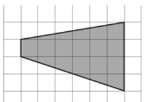
\includegraphics[align=t, width=\linewidth]{../pics/G101M8L5-4}
		\end{minipage}
		\item 
		\begin{minipage}[t]{\bodywidth}
			На рисунке показано, как выглядит колесо с \(7\) спицами. Сколько будет спиц в колесе, если угол между соседними спицами в нем будет равен \(20 \degree \)?
		\end{minipage}
		\hspace{0.02\linewidth}
		\begin{minipage}[t]{\picwidth}
			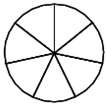
\includegraphics[align=t, width=\linewidth]{../pics/G101M8L5-5}
		\end{minipage}
		%11
		\item 
		\begin{minipage}[t]{\bodywidth}
			Плоскость, проходящая через точки \(A\), \(B\) и \(C\), разбивает куб на два многогранника. Сколько вершин у получившегося многогранника с большим числом граней?
		\end{minipage}
		\hspace{0.02\linewidth}
		\begin{minipage}[t]{\picwidth}
			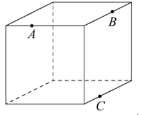
\includegraphics[align=t, width=\linewidth]{../pics/G101M8L5-6}
		\end{minipage}
		%12
		\item В прямоугольном треугольнике \(ABC\) внешний угол при вершине \(A\) равен \(120\degree \). Катет \(AC = 17\). Найдите гипотенузу \(AB\).
		%13
		\item 
		\begin{minipage}[t]{\bodywidth}
			В основании прямой призмы лежит прямоугольный треугольник, катеты которого равны \(3\) и \(16\). Найдите объем призмы, если ее высота равна \(3\).
		\end{minipage}
		\hspace{0.02\linewidth}
		\begin{minipage}[t]{\picwidth}
			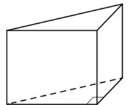
\includegraphics[align=t, width=\linewidth]{../pics/G101M8L5-7}
		\end{minipage}
		\item Найдите значение выражения: \( 4,1 \cdot 7,7 + 0,86 \)
		\item Товар на распродаже уценили на \(30\%\), при этом он стал стоить \(350\) рублей. Сколько рублей стоит товар до распродажи?
		\item Найдите значение выражения: \( (\sqrt{10}-2\sqrt{3})(\sqrt{10}+2\sqrt{3}) \)
		\item Найдите корень уравнения: \(3^{x-8}=\dfrac{ 1 }{ 9 }\)
		\item Каждому из четырѐх чисел в левом столбце соответствует отрезок, которому он принадлежит. Установите соответствие между числами и отрезками из правого столбца. \\ \\
		\begin{minipage}[t]{0.58\linewidth}
			\textbf{Числа:}
			\begin{tasks}
				\task \( \log_235 \)
				\task \( \dfrac{ 7 }{4  } \)
				\task \( \sqrt{13} \)
				\task \( 0,39^{-1} \)
			\end{tasks}
		\end{minipage}
		\hspace{0.05\linewidth}
		\begin{minipage}[t]{\textwidth}
			\textbf{Отрезки:}
			\begin{tasks}
				\task \( [1;2] \)
				\task \( [2;3] \)
				\task \( [3;4] \)
				\task \( [5;6] \)
			\end{tasks}
		\end{minipage}
		\item Найдите четырехзначное число, кратное \(88\), все цифры которого различны и четны. В ответе укажите какое-нибудь одно такое число.
		\item Первую треть трассы автомобиль ехал со скоростью \(60\) км/ч, вторую треть --- со скоростью \(120\) км/ч, а последнюю --- со скоростью \(110\) км/ч. Найдите среднюю скорость автомобиля на протяжении всего пути. Ответ дайте в км/ч.
		\item Петя меняет маленькие фишки на большие. За один обмен он получает \(3\) большие фишки, отдав \(10\) маленьких. До обменов у Пети было \(100\) фишек (среди них были и большие, и маленькие), а после стало \(65\). Сколько обменов он совершил?
	\end{listofex}
\end{class}
%END_FOLD

%BEGIN_FOLD % ====>>_____ Занятие 6 _____<<====
\begin{class}[number=6]
	\begin{listofex}
		%1
		\item В книге Елены Молоховец «Подарок молодым хозяйкам» имеется рецепт пирога с черносливом. Для пирога на \(10\) человек следует взять \(\dfrac{ 1 }{ 10 }\) фунта чернослива. Сколько граммов чернослива следует взять для пирога, рассчитанного на \(3\) человек? Считайте, что \(1\) фунт равен \(0,4\) кг.
		%2
		\item Установите соответствие между величинами и их возможными значениями: к каждому элементу первого столбца подберите соответствующий элемент из второго столбца. \\
		\begin{minipage}[t]{0.58\linewidth}
			\textbf{Величины:}
			\begin{tasks}
				\task объём воды в Азовском море
				\task объём ящика с инструментами
				\task объём грузового отсека транспортного самолёта
				\task объём бутылки растительного масла
			\end{tasks}
		\end{minipage}
		\hspace{0.05\linewidth}
		\begin{minipage}[t]{\textwidth}
			\textbf{Возможные значения:}
			\begin{tasks}
				\task \(150\) м\(^3\)
				\task \(1\) л
				\task \(76\) л
				\task \(256\) км\(^3\)
			\end{tasks}
		\end{minipage}
		%3
		\item
		\begin{minipage}[t]{0.5\linewidth}
			На рисунке жирными точками показана цена нефти на момент закрытия биржевых торгов во все рабочие дни с \(17\) по \(31\) августа \(2004\) года. По горизонтали указываются числа месяца, по вертикали --- цена барреля нефти в долларах США. Для наглядности жирные точки на рисунке соединены линией. Определите по рисунку наименьшую цену нефти на момент закрытия торгов в указанный период (в долларах США за баррель).
		\end{minipage}
		\hspace{0.02\linewidth}
		\begin{minipage}[t]{0.45\linewidth}
			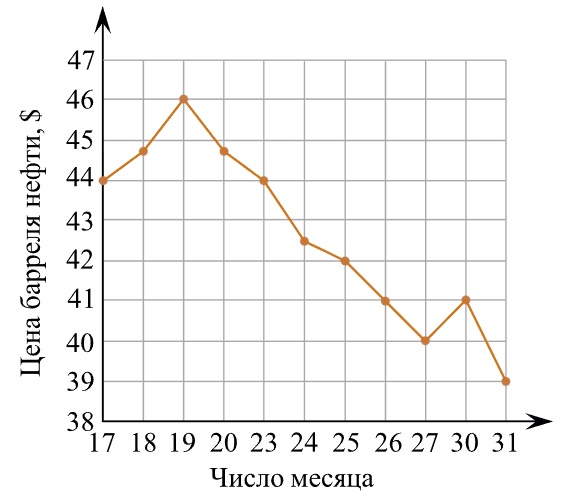
\includegraphics[align=t, width=\linewidth]{../pics/G101M8L6-1}
		\end{minipage}
		%4
		\item В фирме «Родник» стоимость (в рублях) колодца из железобетонных колец рассчитывается по формуле \(С=6000+4100 \cdot n \), где \(n\) --- число колец, установленных при рытье колодца. Пользуясь этой формулой, рассчитайте стоимость колодца из \(5\) колец.
		%5
		\item В фирме такси в данный момент свободно \(20\)  машин: \(10\)  черных, \(2\)  желтых и \(8\) зеленых. По вызову выехала одна из машин, случайно оказавшаяся ближе всего к заказчице. Найдите вероятность того, что к ней приедет зеленое такси.
		%6
		\item 
		\begin{minipage}[t]{\linewidth}
			Для транспортировки \(45\) тонн груза на \(1300\) км можно воспользоваться услугами одной из трех фирм-перевозчиков. Стоимость перевозки и грузоподъемность автомобилей для каждого перевозчика указана в таблице. Сколько рублей придется заплатить за самую дешевую перевозку?
		\end{minipage}
		\hspace{0.02\linewidth}
		\begin{minipage}[t]{\linewidth}
			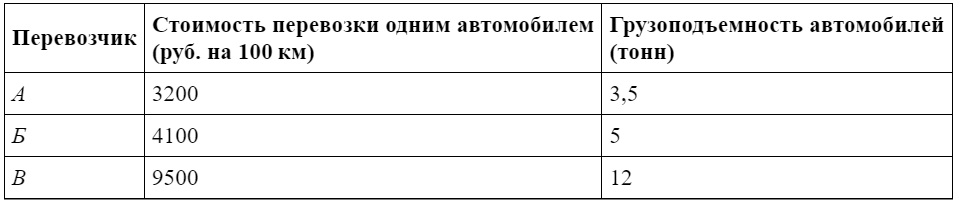
\includegraphics[align=t, width=\linewidth]{../pics/G101M8L6-2}
		\end{minipage}
		%7
		\item 
		\begin{minipage}[t]{\linewidth}
			Установите соответствие между графиками линейных функций и угловыми коэффициентами прямых.
		\end{minipage}
		\hspace{0.02\linewidth}
		\\
		\textbf{Графики:}
		\\
		\begin{minipage}[t]{\linewidth}
			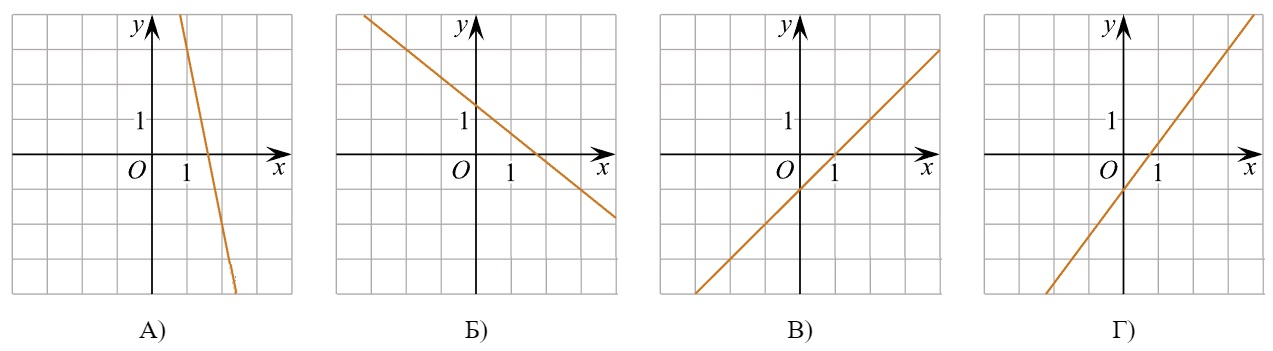
\includegraphics[align=t, width=\linewidth]{../pics/G101M8L6-3}
		\end{minipage}
		\\
		\\
		\textbf{Угловые коэффициенты:}
		\begin{tasks}(4)
			\task \( \dfrac{ 4 }{ 3 } \)
			\task \( -5 \)
			\task \( -0,8 \)
			\task \( 1 \)
		\end{tasks}
		%8
		\item В городе \(X\) в \(2013\) году мальчиков родилось больше, чем девочек. Мальчиков чаще всего называли Андрей, а девочек --- Мария. Выберите утверждения, которые следуют из приведённых данных. Среди рождённых в \(2013\) году в городе \(X\):
		\begin{tasks}
			\task девочек с именем Мария больше, чем с именем Светлана.
			\task мальчиков с именем Николай больше, чем с именем Аристарх.
			\task хотя бы одного из родившихся мальчиков назвали Андреем.
			\task мальчиков с именем Андрей больше, чем девочек с именем Мария.
		\end{tasks}
		%9
		\item
		\begin{minipage}[t]{0.68\linewidth}
			Найдите площадь трапеции, изображенной на клетчатой бумаге с размером клетки \(1\) см на \(1\) см (см. рис.). Ответ дайте в квадратных сантиметрах.
		\end{minipage}
		\hspace{0.02\linewidth}
		\begin{minipage}[t]{0.27\linewidth}
			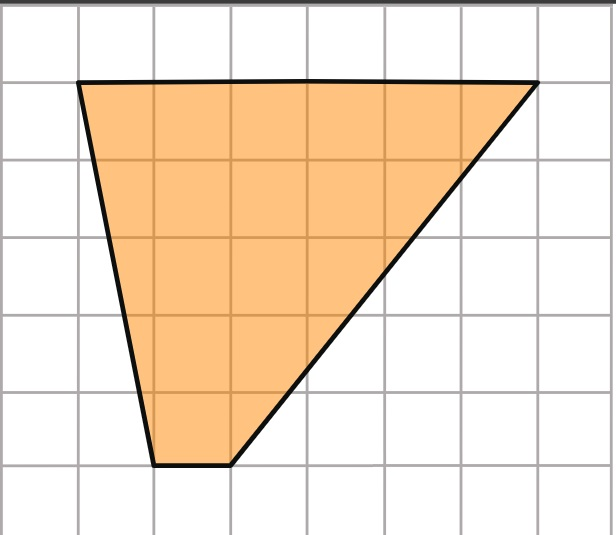
\includegraphics[align=t, width=\linewidth]{../pics/G101M8L6-4}
		\end{minipage}
		%10
		\item
		\begin{minipage}[t]{0.68\linewidth}
			Перила лестницы дачного дома для надёжности укреплены посередине вертикальным столбом. Найдите высоту \(l\) этого столба, если наименьшая высота \(h_1\) перил относительно земли равна \(1,5\) м, а наибольшая \(h_2\) равна \(2,5\) м. Ответ дайте в метрах.
		\end{minipage}
		\hspace{0.02\linewidth}
		\begin{minipage}[t]{0.27\linewidth}
			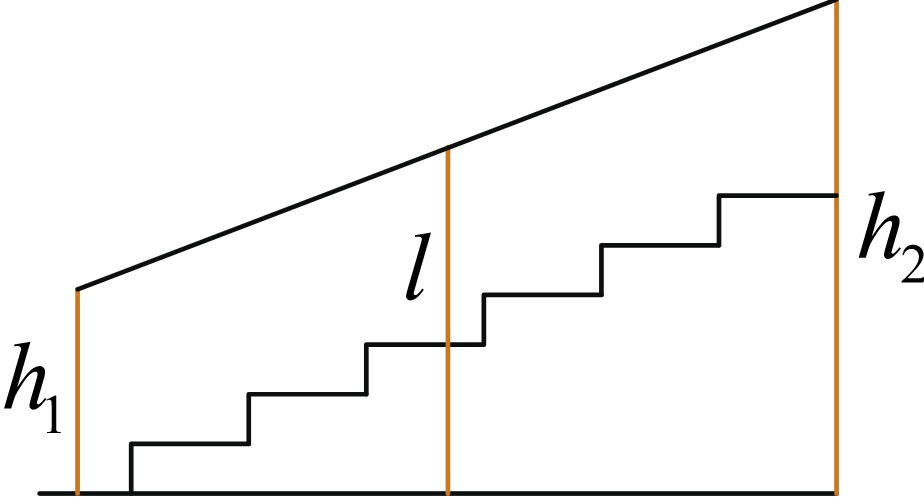
\includegraphics[align=t, width=\linewidth]{../pics/G101M8L6-5}
		\end{minipage}
		%11
		\item
		\begin{minipage}[t]{0.70\linewidth}
			В бак, имеющий форму правильной четырёхугольной призмы со стороной основания, равной \(20\) см, налита жидкость. Для того чтобы измерить объём детали сложной формы, её полностью погружают в эту жидкость. Найдите объём детали, если уровень жидкости в баке поднялся на \(20\) см. Ответ дайте в кубических сантиметрах
		\end{minipage}
		\hspace{0.02\linewidth}
		\begin{minipage}[t]{0.16\linewidth}
			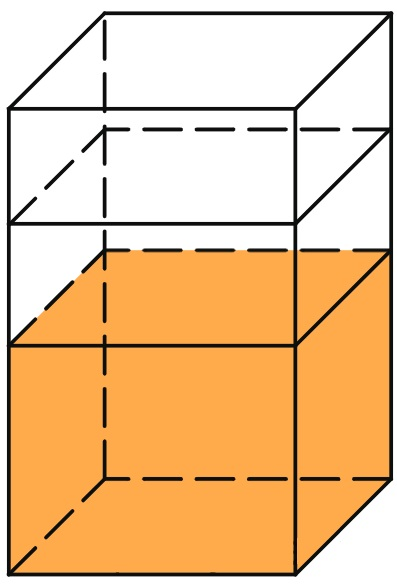
\includegraphics[align=t, width=\linewidth]{../pics/G101M8L6-6}
		\end{minipage}
		%12
		\item В треугольнике \(ABC\): \(AC=BC, AB=8, \tg A = \dfrac{ 33 }{ 4\sqrt{33} }\). Найдите \(AC\).
		%13
		\item Объём конуса равен \(50\pi \), а его высота равна \(6\). Найдите радиус основания конуса.
		%14
		\item Найдите значение выражения: \(-\dfrac{ 9 }{ 25 }+0,21 \cdot \dfrac{ 8 }{ 3 }\).
		%15
		\item Футболка стоила \(800\) рублей. После снижения цены она стала стоить \(680\) рублей. На сколько процентов была снижена цена на футболку?
		%16
		\item Найдите значение выражения: \( \dfrac{ (9^{-3})^2 }{ 9^{-8} } \)
		%17
		\item Найдите корень уравнения: \(\dfrac{ 1 }{ \sqrt{x} }=\dfrac{ 1 }{ 5 }\)
		\newpage
		%18
		\item Каждому из четырёх неравенств в левом столбце соответствует одно из решений из правого столбца. Установите соответствие между неравенствами и множествами их решениями. \\
		\begin{minipage}[t]{0.55\linewidth}
			\textbf{Неравенства:}
			\begin{tasks}
				\task \( \log_2 x >0 \)
				\task \( 2^{-x} > 2 \)
				\task \( \dfrac{ x }{ x-1 }<0 \)
				\task \( \dfrac{ 1 }{ x(x-1) }>0 \)
			\end{tasks}
		\end{minipage}
		\hspace{0.02\linewidth}
		\begin{minipage}[t]{0.4\linewidth}
			\textbf{Решения:}
			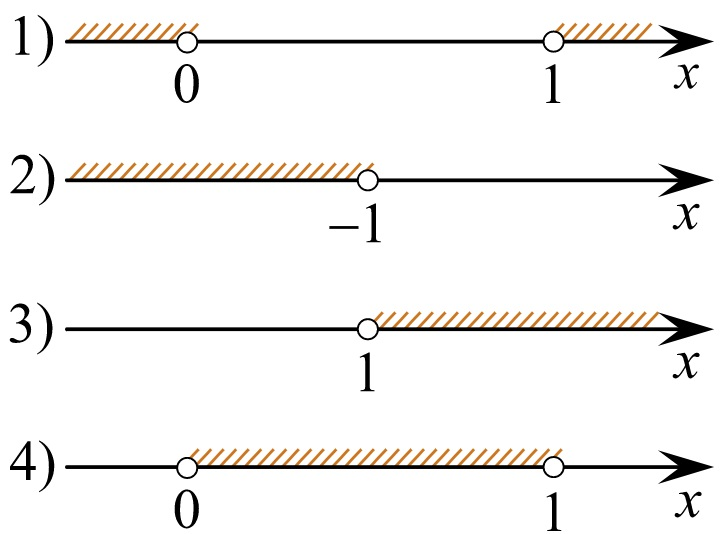
\includegraphics[align=t, width=\linewidth]{../pics/G101M8L6-7}
		\end{minipage}
		\item Найдите четырёхзначное число, кратное \(22\), произведение цифр которого равно \(24\). В ответе укажите какое-нибудь одно такое число.
		\item Имеется два сплава. Первый сплав содержит \(10\%\) никеля, второй --- \(30\%\) никеля. Из этих двух сплавов получили третий сплав массой \(200\) кг, содержащий \(25\%\) никеля. На сколько килограммов масса первого сплава меньше массы второго?
		\item На поверхности глобуса фломастером проведены \(12\) параллелей и \(22\) меридиана. На сколько частей проведённые линии разделили поверхность глобуса? Меридиан --- это дуга окружности, соединяющая Северный и Южный полюсы. Параллель --- это окружность, лежащая в плоскости, параллельной плоскости экватора.
	\end{listofex}
\end{class}
%END_FOLD

%BEGIN_FOLD % ====>>_ Домашняя работа 3 _<<====
\begin{homework}[number=3]
	\begin{listofex}
		\item Больному прописано лекарство, которое нужно пить по \(0,5\) г \(3\) раза в день в течение \(21\) дня. В одной упаковке \(10\) таблеток лекарства по \(0,5\) г. Какого наименьшего количества упаковок хватит на весь курс лечения?
		%2
		\item Установите соответствие между величинами и их возможными значениями: к каждому элементу первого столбца подберите соответствующий элемент из второго столбца. \\
		\begin{minipage}[t]{0.58\linewidth}
			\textbf{Величины:}
			\begin{tasks}
				\task площадь одной страницы учебника
				\task площадь территории республики Карелия
				\task площадь одной стороны монеты
				\task площадь бадминтонной площадки
			\end{tasks}
		\end{minipage}
		\hspace{0.05\linewidth}
		\begin{minipage}[t]{\textwidth}
			\textbf{Возможные значения:}
			\begin{tasks}
				\task \(81,7\) кв. м
				\task \(330\) кв. см
				\task \(180,5\) тыс. кв. км
				\task \(300\) кв. мм
			\end{tasks}
		\end{minipage}
		%3
		\item
		\begin{minipage}[t]{0.5\linewidth}
			На диаграмме показана среднемесячная температура в Нижнем Новгороде (Горьком) за каждый месяц \(1994\) года. По горизонтали указываются месяцы, по вертикали --- температура в градусах Цельсия. Определите по диаграмме наименьшую среднемесячную температуру в \(1994\) году. Ответ дайте в градусах Цельсия.
		\end{minipage}
		\hspace{0.02\linewidth}
		\begin{minipage}[t]{0.45\linewidth}
			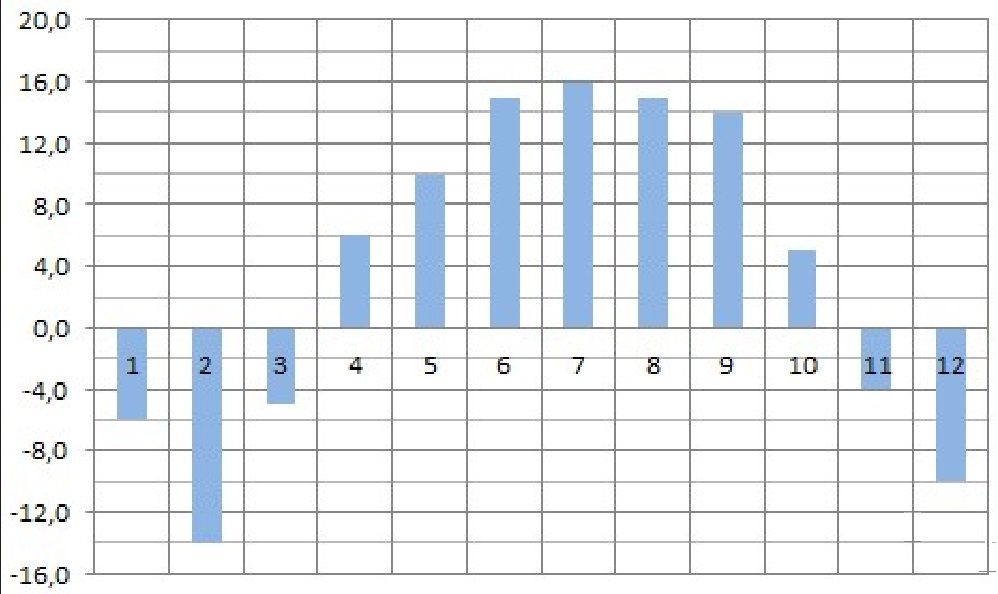
\includegraphics[align=t, width=\linewidth]{../pics/G101M8H3-3}
		\end{minipage}
		\item В фирме «Эх, прокачу!» стоимость поездки на такси (в рублях) рассчитывается по формуле \(C=150+11\cdot (t-5)\), где \(t\) --- длительность поездки, выраженная в минутах \((t>5)\). Пользуясь этой формулой, рассчитайте стоимость \(8\)-минутной поездки.
		\item Перед началом футбольного матча судья бросает монетку, чтобы определить, какая из команд начнёт игру с мячом. Команда «Физик» играет три матча с разными командами. Найдите вероятность того, что в этих играх «Физик» выиграет жребий ровно два раза.
		%6
		\item 
		\begin{minipage}[t]{\linewidth}
			Для изготовления книжных полок требуется заказать \(48\) одинаковых стекол в одной из трех фирм. Площадь каждого стекла \(0,25\) м\(^2\). В таблице приведены цены на стекло, а также на резку стекол и шлифовку края. Сколько рублей будет стоить самый дешевый заказ?
		\end{minipage}
		\hspace{0.02\linewidth}
		\begin{minipage}[t]{\linewidth}
			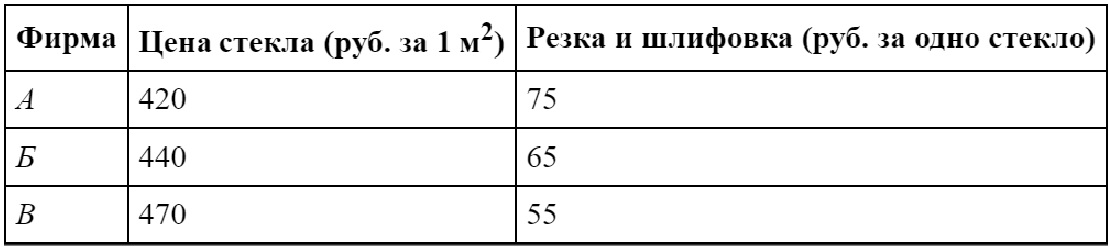
\includegraphics[align=t, width=\linewidth]{../pics/G101M8H3-6}
		\end{minipage}
		%7
		\item 
		\begin{minipage}[t]{0.46\linewidth}
			На рисунке точками изображено число родившихся мальчиков и девочек за каждый календарный месяц \(2013\) года в городском роддоме. По горизонтали указываются месяцы, по вертикали --- количество родившихся мальчиков и девочек (по отдельности). Для наглядности точки соединены линиями.
		\end{minipage}
		\hspace{0.02\linewidth}
		\begin{minipage}[t]{0.5\linewidth}
			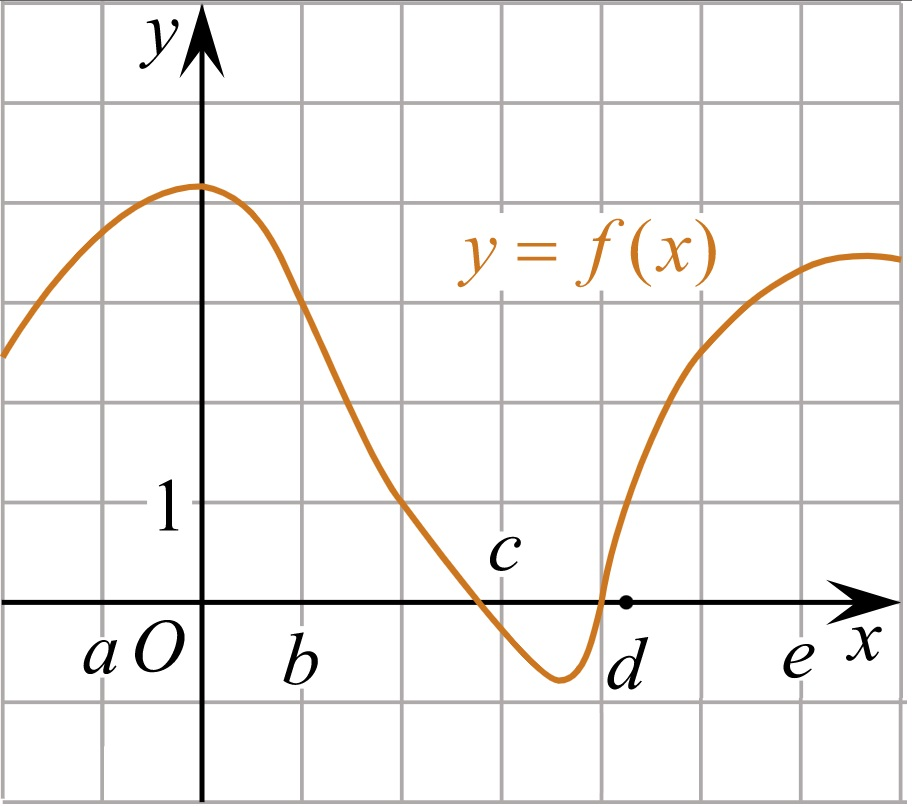
\includegraphics[align=t, width=\linewidth]{../pics/G101M8H3-7}
		\end{minipage}
		\\
		\\
		\textbf{Периоды времени:}
		\begin{tasks}(4)
			\task 1-й квартал года
			\task 2-й квартал года
			\task 3-й квартал года
			\task 4-й квартал года
		\end{tasks}
		\textbf{Характеристика рождаемости:}
		\begin{tasks}
			\task рождаемость мальчиков превышала рождаемость девочек
			\task рождаемость девочек росла
			\task рождаемость девочек снижалась
			\task разность между числом родившихся мальчиков и числом родившихся девочек в один из месяцев этого периода достигает наибольшего значения за год
		\end{tasks}
		\item Средний балл выпускника школы, сдавшего ЕГЭ по четырём предметам, составляет \(75\). Самый низкий результат он показал по математике --- \(66\) баллов (по остальным экзаменам баллы выше). Выберите утверждения, которые следуют из приведённых данных.
		\begin{tasks}
			\task Средний балл по трём экзаменам, кроме математики, равен \(78\)
			\task Минимальный балл по любому из трёх предметов, не считая математики, больше \(75\)
			\task Ни по одному предмету выпускник не получил \(100\) баллов
			\task По какому-то предмету выпускник получил больше \(76\) баллов
		\end{tasks}
		%9
		\item
		\begin{minipage}[t]{0.68\linewidth}
			Найдите площадь четырехугольника, изображенного на клетчатой бумаге с размером клетки \(1\) см на \(1\) см (см. рис.). Ответ дайте в квадратных сантиметрах.
		\end{minipage}
		\hspace{0.02\linewidth}
		\begin{minipage}[t]{0.27\linewidth}
			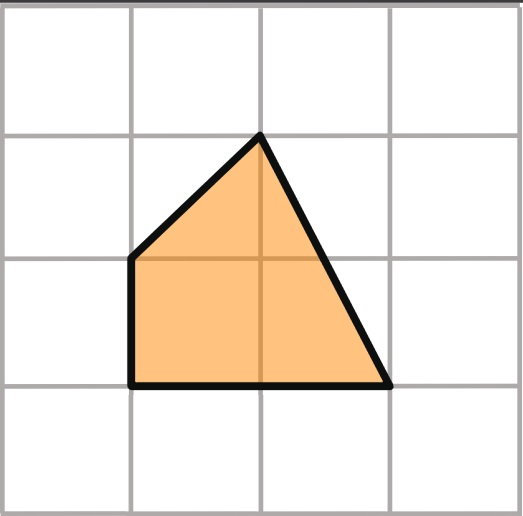
\includegraphics[align=t, width=\linewidth]{../pics/G101M8H3-9}
		\end{minipage}
		%10
		\item
		\begin{minipage}[t]{0.68\linewidth}
			Дачный участок имеет форму прямоугольника со сторонами \(20\) метров и \(30\) метров. Хозяин планирует обнести его забором и разделить таким же забором на две части, одна из которых имеет форму квадрата. Найдите общую длину забора в метрах.
		\end{minipage}
		\hspace{0.02\linewidth}
		\begin{minipage}[t]{0.27\linewidth}
			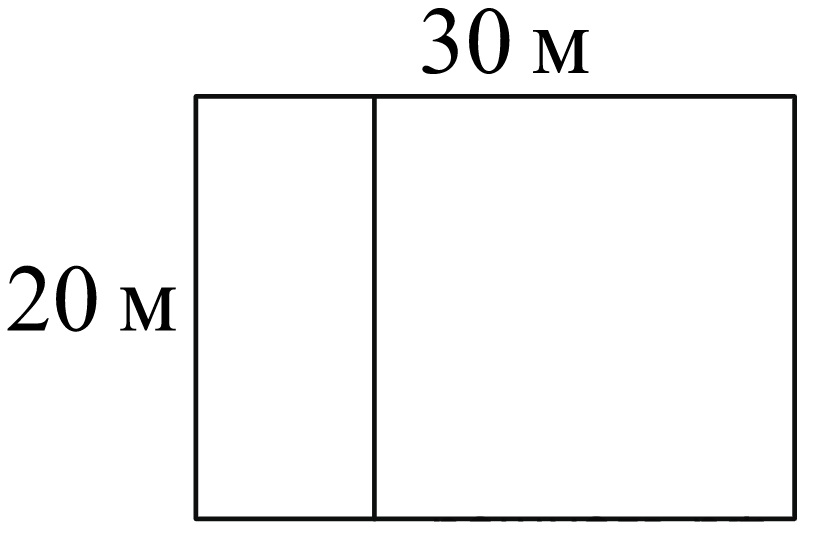
\includegraphics[align=t, width=\linewidth]{../pics/G101M8H3-10}
		\end{minipage}
		%11
		\item
		\begin{minipage}[t]{0.68\linewidth}
			В бак, имеющий форму прямой призмы, налито \(12\) л воды. После полного погружения в воду детали, уровень воды в баке поднялся в \(1,5\) раза. Найдите объём детали. Ответ дайте в кубических сантиметрах, зная, что в одном литре \(1000\) кубических сантиметров.
		\end{minipage}
		\hspace{0.02\linewidth}
		\begin{minipage}[t]{0.27\linewidth}
			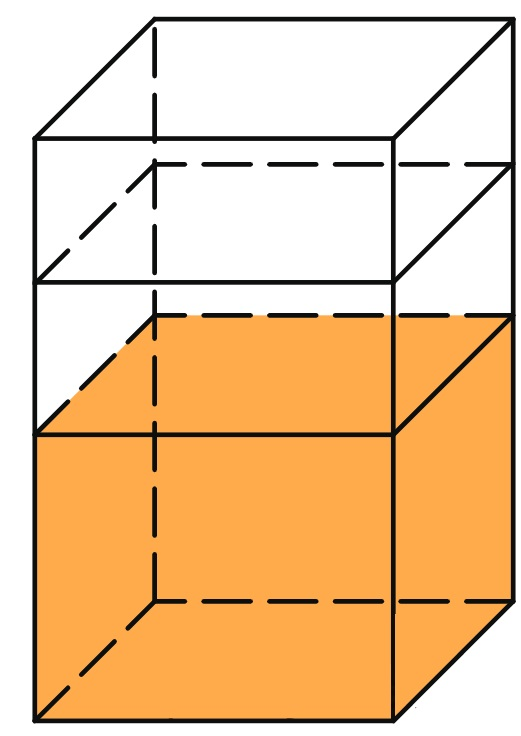
\includegraphics[align=t, width=\linewidth]{../pics/G101M8H3-11}
		\end{minipage}
		\item Катеты прямоугольного треугольника равны \(6\) и \(8\). Найдите наибольшую среднюю линию треугольника.
		\item Два ребра прямоугольного параллелепипеда равны \(7\) и \(4\), а объём параллелепипеда равен \(140\). Найдите площадь поверхности этого параллелепипеда.
		\item Найдите значение выражения: \(\dfrac{ 14 }{15  }:\dfrac{ 7 }{ 3 }-0,5\)
		\item Только \(94\%\) из \(27 500\) выпускников города правильно решили задачу \(B1\). Сколько человек правильно решили задачу \(B1\)?
		\item Найдите значение выражения: \(\dfrac{ 4^{3,5}\cdot 5^{2,5} }{ 20^{1,5} }\).
		\item Найдите корень уравнения: \(3^{2x-5}\cdot 3^{2x-3}=\dfrac{ 1 }{ 81 }\).
		%18
		\item Каждому из четырёх неравенств в левом столбце соответствует одно из решений в правом столбце. Установите соответствие между неравенствами и их решениями. \\
		\begin{minipage}[t]{0.55\linewidth}
			\textbf{Неравенства:}
			\begin{tasks}
				\task \( \log_2 x >1 \)
				\task \( \log_2 x >-1 \)
				\task \( \log_2 x <1 \)
				\task \(\log_2 x <-1 \)
			\end{tasks}
		\end{minipage}
		\hspace{0.02\linewidth}
		\begin{minipage}[t]{0.4\linewidth}
			\textbf{Решения:}
			\begin{tasks}
				\task \( 0<x<0,5 \)
				\task \( x>2 \)
				\task \( x>0,5 \)
				\task \( 0<x<2 \)
			\end{tasks}
		\end{minipage}
		\item Цифры четырёхзначного числа, кратного \(5\), записали в обратном порядке и получили второе четырёхзначное число. Затем из первого числа вычли второе и получили \(1458\). Приведите ровно один пример такого числа.
		\item Смешали некоторое количество \(15\)-процентного раствора некоторого вещества с таким же количеством \(19\)-процентного раствора этого вещества. Сколько процентов составляет концентрация получившегося раствора?
		\item В доме всего \(14\) квартир с номерами от \(1\) до \(14\). В каждой квартире живёт не менее \(1\) и не более \(4\) человек. В квартирах с \(1\)-й по \(12\)-ю включительно живёт суммарно \(14\) человек, а в квартирах с \(11\)-й по \(14\)-ю включительно живёт суммарно \(12\) человек. Сколько всего человек живут в этом доме?
	\end{listofex}
\end{homework}
%END_FOLD

%BEGIN_FOLD % ====>>_____ Занятие 7 _____<<====
\begin{class}[number=7]
	\begin{listofex}
		%20.2 n1,2,8
		\item Из двух городов, расстояние между которыми равно \(560\) км, навстречу друг другу одновременно выехали два автомобиля. Через сколько часов автомобили встретятся, если их скорости равны \(65\) км/ч и \(75\) км/ч?
		\item Из пункта \(A\) в пункт \(B\) одновременно выехали два автомобиля. Первый проехал с постоянной скоростью весь путь. Второй проехал первую половину пути со скоростью \(24\) км/ч, а вторую половину пути --- со скоростью, на \(16\) км/ч большей скорости первого, в результате чего прибыл в пункт B одновременно с первым автомобилем. Найдите скорость первого автомобиля. Ответ дайте в км/ч.
		
		%20.4 n1,3
		\item Моторная лодка прошла против течения реки \(112\) км и вернулась в пункт отправления, затратив на обратный путь на \(6\) часов меньше. Найдите скорость течения, если скорость лодки в неподвижной воде равна \(11\) км/ч. Ответ дайте в км/ч.
		\item Моторная лодка в \(10:00\) вышла из пункта \(A\) в пункт \(B\), расположенный в \(30\) км от \(A\). Пробыв в пункте \(B\) \(2\) часа \(30\) минут, лодка отправилась назад и вернулась в пункт \(A\) в \(18:00\). Определите (в км/ч) собственную скорость лодки, если известно, что скорость течения реки \(1\) км/ч.
		%20.3 n1,3
		\item Два мотоциклиста стартуют одновременно в одном направлении из двух диаметрально противоположных точек круговой трассы, длина которой равна \(14\) км. Через сколько минут мотоциклисты поравняются в первый раз, если скорость одного из них на \(21\) км/ч больше скорости другого?
		\item Из пункта \(A\) круговой трассы выехал велосипедист, а через \(30\) минут следом за ним отправился мотоциклист. Через \(10\) минут после отправления он догнал велосипедиста в первый раз, а еще через \(30\) минут после этого догнал его во второй раз. Найдите скорость мотоциклиста, если длина трассы равна \(30\) км. Ответ дайте в км/ч.
		
		%\item Плот и лодка движутся навстречу друг другу по реке. Они находятся на расстоянии \(20\) км друг другу по реке. Они находятся на расстоянии \(20\) км друг от друга. Через какое время они встретятся, если собственная скорость лодки \(8\) км/ч, а скорость течения реки \(2\) км/ч?
		%20.1 n7,8,9
		\item Имеется два сплава. Первый содержит \(15\%\) никеля, второй --- \(35\%\) никеля. Из этих двух сплавов получили третий сплав массой \(140\) кг, содержащий \(30\%\) никеля. На сколько килограммов масса первого сплава была меньше массы второго?
		\item Сплав золота и серебра массой \(4\) кг содержит \(30\%\) золота. К нему добавили другой сплав золота и серебра, содержащий \(55\%\) золота и получили сплав, содержащий \(40\%\) золота. Какова масса нового сплава?
		\item В сосуд, содержащий \(5\) литров \(12\)-процентного водного раствора некоторого вещества, добавили \(7\) литров воды. Сколько процентов составляет концентрация получившегося раствора?
		\item Смешали \(4\) литра \(15\)-процентного водного раствора некоторого вещества с \(6\) литрами \(25\)-процентного водного раствора этого же вещества. Сколько процентов составляет концентрация получившегося раствора?
		\item Смешали некоторое количество \(15\)-процентного раствора некоторого вещества с таким же количеством \(19\)-процентного раствора этого вещества. Сколько процентов составляет концентрация получившегося раствора?
		
	\end{listofex}
\end{class}
%END_FOLD

%BEGIN_FOLD % ====>>_ DZ4 _<<====
\begin{homework}[number=4]
	\begin{listofex}
		\item Из двух городов, расстояние между которыми равно \(320\) км, навстречу друг другу одновременно выехали два автомобиля. Через сколько часов автомобили встретятся, если их скорости равны \(75\) км/ч и \(85\) км/ч?
		\item Из пункта \(A\) в пункт \(B\) одновременно выехали два автомобиля. Первый проехал с постоянной скоростью весь путь. Второй проехал первую половину пути со скоростью, меньшей скорости первого на \(13\) км/ч, а вторую половину пути --- со скоростью \(78\) км/ч, в результате чего прибыл в пункт \(B\) одновременно с первым автомобилем. Найдите скорость первого автомобиля, если известно, что она больше \(48\) км/ч. Ответ дайте в км/ч.
		\item Моторная лодка прошла против течения реки \(255\) км и вернулась в пункт отправления, затратив на обратный путь на \(2\) часа меньше. Найдите скорость лодки в неподвижной воде, если скорость течения равна \(1\) км/ч. Ответ дайте в км/ч.
		\item В сосуд, содержащий \(8\) литров \(11\)-процентного водного раствора некоторого вещества, добавили \(3\) литра воды. Сколько процентов составляет концентрация получившегося раствора?
		\item Смешали некоторое количество \(13\)-процентного раствора некоторого вещества с таким же количеством \(17\)-процентного раствора этого вещества. Сколько процентов составляет концентрация получившегося раствора?
		\item Смешали \(8\) литров \(25\)-процентного водного раствора некоторого вещества с \(12\) литрами \(20\)-процентного водного раствора этого же вещества. Сколько процентов составляет концентрация получившегося раствора?
		\item 
		\begin{minipage}[t]{\bodywidth}
			Найдите площадь поверхности многогранника и объём куба, если его сторона равна \(3\sqrt{2}\) см.
		\end{minipage}
		\hspace{0.02\linewidth}
		\begin{minipage}[t]{\picwidth}
			\includegraphics[align=t, width=\linewidth]{\picpath/../../bank/graphs/graph_gleb/Spoverxn/cube}
		\end{minipage}
		\item 
		\begin{minipage}[t]{\bodywidth}
			Найдите площадь поверхности пространственного креста, изображенного на рисунке и составленного из кубов, сторона которого равна \(3\) см.
		\end{minipage}
		\hspace{0.02\linewidth}
		\begin{minipage}[t]{\picwidth}
			\includegraphics[align=t, width=\linewidth]{\picpath/../../bank/graphs/graph_gleb/Spoverxn/6cubes}
		\end{minipage}
		
		\item 
		\begin{minipage}[t]{\bodywidth}
			Найдите площадь поверхности многогранника, изображенного на рисунке (все двугранные углы прямые).
		\end{minipage}
		\hspace{0.02\linewidth}
		\begin{minipage}[t]{\picwidth}
			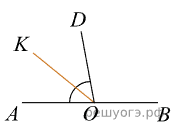
\includegraphics[align=t, width=\linewidth]{\picpath/../../bank/graphs/graph_gleb/Spoverxn/1}
		\end{minipage}
	
	\item 
	\begin{minipage}[t]{\bodywidth}
		Найдите объем и площадь поверхности многогранника, изображенного на рисунке (все двугранные углы прямые).
	\end{minipage}
	\hspace{0.02\linewidth}
	\begin{minipage}[t]{\picwidth}
		\includegraphics[align=t, width=\linewidth]{\picpath/../../bank/graphs/graph_gleb/Spoverxn/2}
	\end{minipage}
\end{listofex}
\end{homework}
%END_FOLD